\chapter{Fairness.}
\label{ch:fairness}
\only<article>{ When machine learning algorithms are applied at scale,
  it can be difficult to imagine what their effects might be. In this
  part of the book, we consider notions of fairness as seen through
  the prism of conditional independence and meritocracy. The first
  notion requires that we look deeper into directed graphical models.
  
  The problem of fairness in machine learning and
  artificial intelligence has only recently been widely
  recognised. When any algorithm is implemented at scale, no matter
  the original objective and whether it is satisfied, it has
  significant societal effects. In particular, even when considering
  the narrow objective of the algorithm, even if it improves it
  overall, it may increase inequality.
  
  In this course we will look at two aspects of fairness. The first
  has to do with disadvantaged populations that form distinct social
  classes due to a shared income stratum, race or gender. The second
  has to do with meritocratic notions of fairness.

  This chapter requires some knowledge of decision theory (See
  Chapter~\ref{ch:decision-problems}) to understand the principles of
  expected utility maximisation and graphical models (See
  Chapter~\ref{ch:graphical-models}) to understand the idea of conditional independence.
}

\section{Introduction.}


\only<article>{ Fairness is a concept that has received much attention
  recently when applied to large-scale algorithmic decision
  making. However, the very concept of fairness is not well-defined
  and encompasses many different ideas. Some of those relate to fair
  treatment of individuals: \emph{Meritocracy} is the idea that people
  should receive rewards according to their merit. \emph{Equal
    treatment} is the related notion that similar people should be
  treated similarly under similar circumstances. Some concepts are
  related more to the treatment of different groups:
  \emph{Proportional representation} is the idea that proportions of
  different groups in society should be reflected in every facet of
  society. Finally \emph{non-discrimination} captures the notion of
  not treating people differently depending on sensitive
  characteristics.  }

\only<presentation>{
  \begin{frame}
    \frametitle{Fairness}
    What is it?
    \begin{itemize}
    \item<2-> \alert{Meritocracy}.
    \item<3-> Proportionality and representation.
    \item<4-> Equal treatment.
    \item<5-> \alert{Non-discrimination}.
    \end{itemize}
  \end{frame}
}

\begin{frame}
  \frametitle{Meritocracy}
  \only<article>{

    Meritocracy embodies the principle that merit should be
    rewarded. A common example are admissions to universities. Some
    type of summary, typically a grade obtained from high school, is
    used to represent the underlying merit of individuals.
  }
  \uncover<2->{
    \begin{example}[College admissions]
      \only<article>{ In this example, we have two students. In terms
        of grades, student $B$ is clearly better. If we can only
        accept one of them, and given no other information, it seems
        like the natural choice is student $B$.  }
      \begin{itemize}
      \item Student $A$ has a grade 4/5 from Gota Highschool.
      \item Student $B$ has a grade 5/5 from Vasa Highschool.
      \end{itemize}
    \end{example}
  }
  \only<article>{Grades, by themselves, are typically insufficient information. It might be that grades from some high-schools are inflated and do not represent the quality of individuals accurately. So, let us suppose we now consider the information.}
  \uncover<3->{
    \begin{example}[Additional information]
      \only<article>{
        In particular, let us suppose that we have statistics on how well students from different high school do, depending on their high school grade.
      }
      \begin{itemize}
      \item 70\% of admitted Gota graduates with 4+ get their degree.
      \item 50\% of admitted Vasa graduates with 5 get their degree.
      \end{itemize}
      \only<article>{
        All other thing being equal, it is now more likely that student $A$ will graduate. So perhaps we should take in $A$ and not $B$.
      }
    \end{example}
  }

  \uncover<4->{We still don't know how a \alert{specific} student will
    do!}

  \only<article>{ I must emphasise that these are only
    statistics, and not necessarily predictive of the students'
    ability.  Ideally, we would like to admit the students that we
    expect to do well, given the information that we have. However,
    this information is typically not enough for us to make reliable
    predictions.  In addition, we might want to also make sure that
    everybody has a chance to obtain a good education. In order to
    achieve this, we might want to promote ethnic or gender equality
    through university admissions.  Unfortunately, there is no ideal
    solution and we must always balance the benefit of individual
    students with that of specific societal groups as well as society
    as a whole.
  }
  

\end{frame}


\only<presentation>{
  \begin{frame}
    \frametitle{Hiring decisions}
    \begin{columns}
      \begin{column}{0.5\textwidth}
        \includegraphics[height=\textheight]{../figures/cmu-headcount}
      \end{column}
      \begin{column}{0.5\textwidth}
        \includegraphics[width=\columnwidth]{../figures/amazon-hiring}
        \\
        \includegraphics[width=\columnwidth]{../figures/recruitement-automation}
      \end{column}
    \end{columns}
  \end{frame}


  \begin{frame}
    \frametitle{Group fairness and proportionality}
    \includegraphics[width=\textwidth]{../figures/genomics-diversity}
    \url{https://qz.com/1367177/}
  \end{frame}

}

\begin{frame}  
  \begin{block}{Solutions}
    \only<article>{These solution methods are not completely exclusive, and can be implemented simultaneously to some extent.}
    \begin{itemize}
    \item<5-> Admit \alert{everybody}? \only<article>{This suggests that everybody is admitted to at least one university, perhaps even their university of choice. However, it requires that there is enough teaching capacity for all students in the first year. Subsequently, we expect the students who were not qualified to drop out. Of course, this is unfair to the qualified students, as it drains resources that could have been used for them.}
    \item<6-> Admit \alert{randomly}? \only<article>{Completely random decisions are not considered fair, because they do not take into account any information. However, randomisation can also be used in conjunction with grades to ensure that everybody has a shot.}
    \item<7-> Use \alert{prediction} of individual academic performance? \only<article>{The more information we have, the better we can predict academic performance. A grade from high school is one indicator, but more data can be used to obtain better predictions. Of course, no prediction is perfect.}
    \item<8-> Should we take into account \alert{group membership} or other population information? \only<article>{For many reasons, students in some groups can perform differently in standardised tests, even though their innate talents may be no different than students not in the group. The classical example of this is high school teachers discouraging girls from mathematics.}
    \end{itemize}
  \end{block}
  
\end{frame}


\only<article>{
  \begin{example}[Hiring decisions.]
    As a further example, consider gender balance in hiring decisions.
    Typically, received applications are screened, so that some
    applicants undergo through an interview process. At the end, some
    of the interviewed applicants will be hired. There are two
    decision points here, with most people being cut off at the first
    point: the screening. To automate this process, Amazon worked on
    resume-screen program.~\footnote{\url{https://www.reuters.com/article/us-amazon-com-jobs-automation-insight-idUSKCN1MK08G}}
    However, this was scrapped after it was discovered that it
    predominantly favoured men. The reason is not entirely clear, but
    it was probably due to the fact that they trained the system on
    their own screening decisions, and given that the tech industry
    predominantly hires men in the first place, women were likely
    rejected in the screening phase. 
  \end{example}
}


b\section{Group fairness.}
\only<article>{ Let us now take a look at concepts of fairness related
  to \emph{group membership}. This includes concepts such as equal
  treatment, equality of opportunity and generally lack of
  discrimination.  The general idea is that we would like for members
  of society to follow trajectories through life that do not strongly
  depend on their membership in sensitive groups. For example, gender
  should not play a role in academic achievement. Ethnic heritage
  should have no influence on annual income. Unfortunately, the
  underlying societal dynamics create situations where group
  membership becomes important.

  In this section, and throughout this chapter, we will imagine that
  an individual is interacting with a system, which makes decisions
  about the individual, such as whether or not to give them a
  loan. These result in a certain outcome , such as the individual
  using the borrowed money to invest in a business and then having a
  particular annual income. Crucially, these outcomes can be
  correlated with group membership, because of societal dynamics. The
  system designer should make sure that not only the system does what
  it intends, such as giving loans to people that are expected to
  repay them, but also that it does not create inequalities between
  different groups. As we will see later, depending on our fairness
  definition, and on the societal dynamics, this is not always easy.
  
}

\begin{frame}
  \frametitle{Bail decisions}

  \only<article>{ For a more detailed
    example, let us consider bail decisions in the US court
    system. When a defendant is charged, the judge has the option to
    either place them in jail pending trial, or set them free, under
    the condition that the defendant pays some amount of 'bail'. The
    amount of bail (if any) is set to deter flight or a relapse.

    This process sometimes includes the use of a software tool called
    \texttt{COMPAS}, which gives risk scores for the possibility of
    flight, recidivism or violent behaviour. These scores are taken
    into account by judges when making decisions.  In some cases, it
    appears as though automating this procedure might lead to better
    outcomes. But is that generally true?
  }


  \only<presentation>{
    \begin{columns}
      \begin{column}{0.5\textwidth}
        \centering
        \begin{tikzpicture}
          \node at (0,0) (judge) {\includegraphics[width=0.3\columnwidth]{../figures/judge}};
          \uncover<2->{
            \node at (-2,-2) (jail) {\includegraphics[width=0.3\columnwidth]{../figures/jail}};
            \draw[->] (judge) -- (jail);
          }
          \uncover<3->{
            \node at (2,-2) (bail) {\includegraphics[width=0.3\columnwidth]{../figures/bail}};
            \draw[->] (judge) -- (bail);
          }

          \uncover<4->{
            \node at (-2,-4) (trial) {\includegraphics[width=0.3\columnwidth]{../figures/trial}};
            \draw[->] (jail) -- (trial);
          }
          \uncover<5->{
            \draw[->] (bail) -- (trial);
          }
          \uncover<6->{
            \node at (2,-4) (arrest) {\includegraphics[width=0.3\columnwidth]{../figures/handcuffs}};
            \draw[->] (bail) -- (arrest);
          }
        \end{tikzpicture}
      \end{column}
      \begin{column}{0.5\textwidth}
        \centering
        \uncover<7->{
          \includegraphics[width=\textwidth]{../figures/judge-fairness}
        }
      \end{column}
    \end{columns}
  }

  \only<article>{In this setting, a defendant $t$ appears before a
    judge with observable features $x_t \in \CX$, and a sensitive group
    variable $z_t \in \CZ$. The judge employs a specific policy $\pol$ to
    select a decision $a_t \in \CA$, with
    \begin{equation}
      \pol(a_t \mid x_t, z_t)
    \end{equation}
    denoting the probability of action $a_t$ given the individual's features, as well as the sensitive variable. We can assume that the policy is fixed ahead of time, and thereafter decisions are made according to the policy.
    After the judge makes their decision, they observe an outcome $y_t$ sampled from some potentially unknown distribution with parameter $\theta$:
    \begin{equation}
      P_\theta(y_t \mid x_t, z_t, a_t), 
    \end{equation}
    denoting the probability of $y_t$ given the individual's features
    and the action taken.

    The choice of policy has to reflect the preferences of the
    decision maker (in this case the judge). In our example, let us
    consider a simple set of actions $\CA = \{0, 1\}$, where a
    defendant is granted $(a_t = 1)$ or denied $(a_t = 0)$ bail.  If a
    defendant is not given bail, they must remain in jail. This costs
    both the government and the defendant, so the judge prefers not to
    deny bail too often.  On the other hand, if the defendant is
    granted bail, there is a chance they will re-offend $(y_t =
    1)$. Consequently, we can define the following utility function\footnote{See Chapter~\ref{ch:decision-problems}}
    for the judge, that roughly reflects those preferences:
    \begin{equation}
      U(a, y) = a - y.
    \end{equation}
    While this weighs the judge's two main concerns equally, we can also imagine different formulations: e.g. if the judge thinks it is much more important to keep people out of jail than to prevent re-offences until trial, they might select a function such as : $U(a, y) = 10a - y$.
    Now, given the parameter $\theta$ of the unknown distribution, the judge can find a decision rule $\pol$ maximising utility in expectation
    \begin{equation}
      \label{eq:expected-utility-judge}
      \E_\param^\pol(U) = \sum_{x,z} P_\theta(x, z) \sum_a \pol(a | x, z) \sum_y P_\theta(y | a, x, z) U(a,y).
    \end{equation}
    If we are estimating the decision rule from some training set, we can simply solve the following maximisation problem:
    \[
      \max_\pol \sum_{t} \sum_a \pol(a | x_t, z_t) U(a,y_t).
    \]
    However, doing so may have unintended effects, as treatment of different groups may be unequal. For that reason, we may have to add explicit fairness constraints to our optimisation problem.
  }
\end{frame}  

\begin{frame}
  \frametitle{Demographic parity and equality of opportunity.}

  \only<article>{Let us take a look at how many individuals are given
    different scores. Figure~\ref{fig:risk-bias} shows the proportions
    of individuals obtaining different risk scores as a function of
    their ethnic group. While the general population, and Caucasians
    in particular, have a distribution sharply concentrated in low
    scores, Black defendants obtain much higher risk scores: they are
    almost as likely to be ranked a 10 as the are to be scored a 1. }
  \begin{figure}[H]
    \begin{columns}
      \begin{column}{0.5\textwidth}
        \centering
        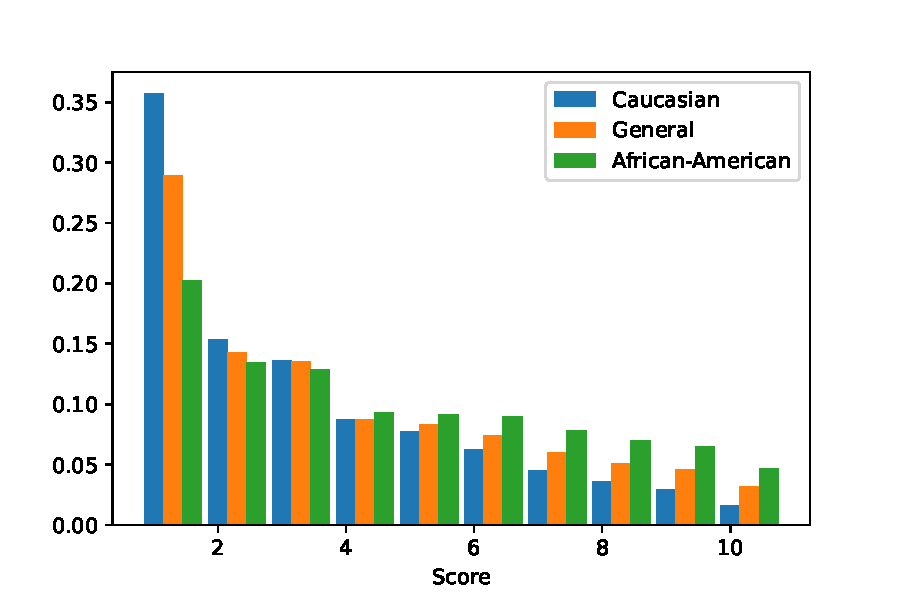
\includegraphics[width=\columnwidth]{../figures/Scores-by-race}      
      \end{column}
    \end{columns}
    \label{fig:risk-bias}
    \caption{Apparent bias in risk scores towards black versus white defendants.}
  \end{figure}
  \only<article>{ Typically, we would like to demographic parity
    across groups, either with respect to the decisions, or with
    respect to the outcomes.  Decision parity is called \emph{equality
      of opportunity} and satisfies the following condition
    \begin{equation}
      \label{eq:equality-opportunity}
      \Pr_\param^\pol(a_t | z_t) =       \Pr_\param^\pol(a_t ).
    \end{equation}
    In other words, the action (risk score, in this case) is
    independent of the group.  As we see in
    Figure~\ref{fig:risk-bias}, these distributions are quite
    different.  The curve for ``General'' corresponds to
    $\Pr_\param^\pol(a_t )$, while the other two curves correspond to
    $\Pr_\param^\pol(a_t | z_t)$ for $z_t$ being Caucasian and
    African-American respectively.
    
    \emph{Demographic parity} instead relates to outcomes. If this
    condition is satisfied, then the probability distribution of
    outcomes is independent of group membership.
        \begin{equation}
      \label{eq:eqality-outcomes}
      \Pr_\param^\pol(y_t | z_t) =       \Pr_\param^\pol(y_t ).
    \end{equation}

  }
\end{frame}

\begin{frame}
  \frametitle{Calibration.}
  
  \only<article>{On the
    other hand, the scores generated by the software seemed to be very
    predictive on whether or not defendants would re-offend,
    independently of their race. Figure~\ref{fig:imrs} shows that, if
    an individual obtains a high score then they are very likely to
    re-offend, and conversely, they are unlikely to re-offend when
    they have a low score. }
  \begin{figure}[H]
    \centering
    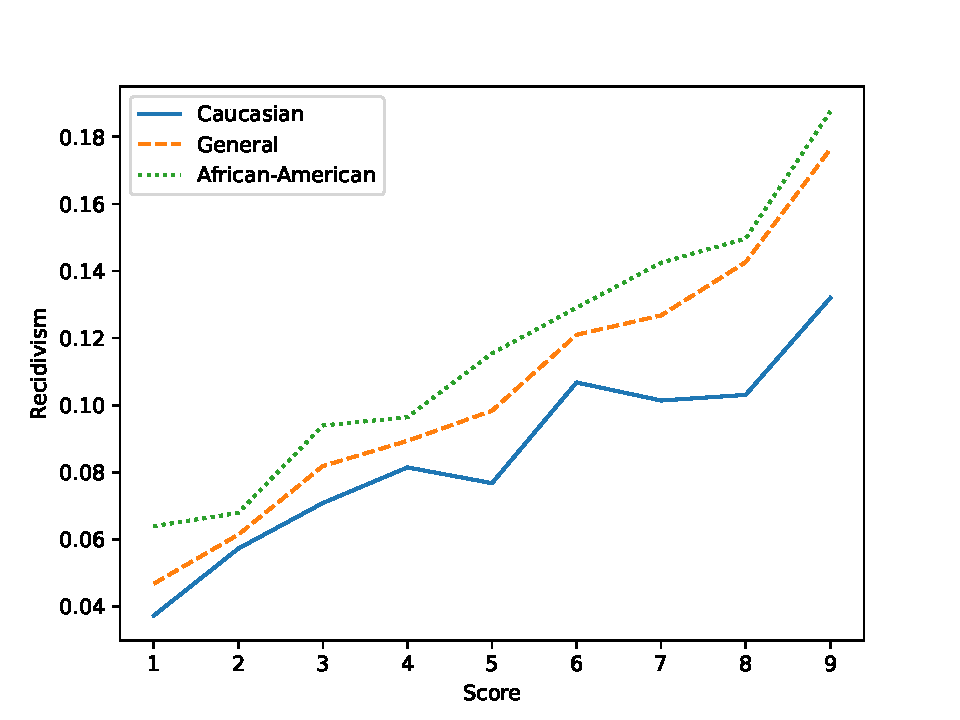
\includegraphics[width=\columnwidth]{../figures/calibration-compas}
    \caption{Recidivism rates by risk score.}
    \label{fig:imrs}
  \end{figure}
  This concept can be quantified in terms of the conditional distribution of outcomes given the score:
  \begin{equation}
    \Pr_\param^\pol(y_t | a_t, z_t) =       \Pr_\param^\pol(y_t | a_t).
    \label{eq:calibration}
  \end{equation}
  This means that $y_t$ is conditionally independent of $z_t$ given
  the score $a_t$. So, in some sense, the score is sufficient for us
  to predict the outcome, and knowing the race does not help us
  predict any better.  
\end{frame}

\begin{frame}
  \frametitle{Balance}
  \only<article>{While the system's predictions seem to be calibrated against the chance of recidivism, this does not mean that race plays no role. Figure~\ref{fig:imrs-risk} breaks down the population in people that re-offended and those that did. For each sub-population, we then plot the proportion of people receiving different scores by race. While people generally have a small probability of obtaining a high risk score, we see that Black defendants obtain much higher scores.}
  
  \begin{figure}[H]
    \centering
    \begin{subfigure}{0.45\textwidth}
      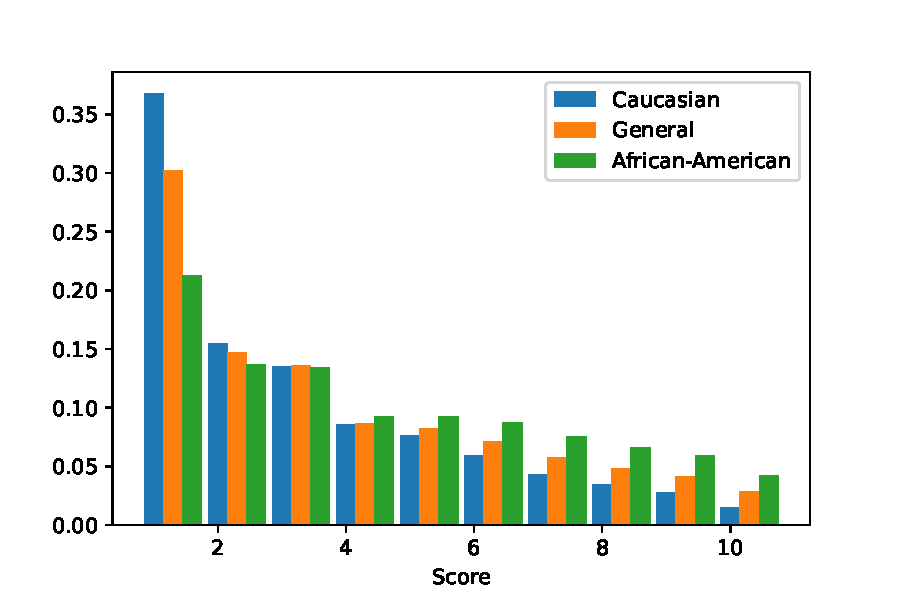
\includegraphics[width=0.95\textwidth]{../figures/balance-non-recidivism-compas}
      \caption{No recidivism}
    \end{subfigure}
    \begin{subfigure}{0.45\textwidth}
      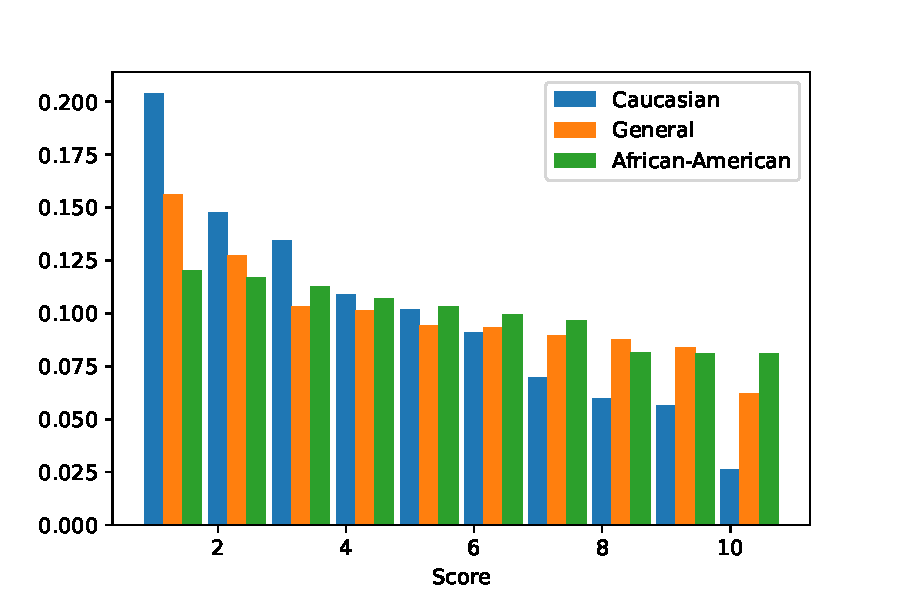
\includegraphics[width=0.95\textwidth]{../figures/balance-recidivism-compas}
      \caption{Recidivism}
    \end{subfigure}
    \caption{Score breakdown based on recidivism rates.}
    \label{fig:imrs-risk}
  \end{figure}
  \only<article>{
    Balance can also be interpreted as a probabilistic condition, of the following form:
    \begin{equation}
      \Pr_\param^\pol(a_t | y_t, z_t) =       \Pr_\param^\pol(a_t | y_t).
      \label{eq:balance}
    \end{equation}
    Here we have that $a_t$ is conditionally independent of $z_t$
    given the outcome $y_t$. So, if we partition the population
    according to their outcome, we should find that given the outcome,
    the distribution of scores is the same no matter what their
    race. However, this is not what the example shows: there is a
    strong dependence on race.  }
  
\end{frame}

\only<presentation>{

  \begin{frame}
    \frametitle{Graphical models and independence}
    \begin{itemize}
    \item Why is it not possible to be fair in all respects?
    \item Different notions of \alert{conditional independence}.
    \item Can only be satisfied rarely simultaneously.
    \end{itemize}
  \end{frame}

}

\only<article>{ How can we explain this discrepancy? We can show that
  in fact, each one of these different measures of bias in our
  decision rules can be seen as a notion of conditional
  independence. Had $z_t$ been an independent variable, i.e. so that
  $P_\param(x,z) = P_\param(x) P_\param(z)$ and
  $P_\param(y | x,a,z) = P_\param(y | x,a)$, then it would have no
  role. Unfortunately, though, it does influence the distributions of
  the other variables.  }


\begin{example}[Classification]
  One setting where the above discussion applies directly are classification problems. There, the outcomes $y$ are simply labels. the decision space $\CA$ is to just predicting a label, and the utility function is the classification accuracy, so that $U(a, y) = \ind{a = y}$. In this setting, $y$ does not directly depend on $a$, since $a$ is just a prediction of the latent label.  More precisely, $y \indep a \mid x$. This allows us to write:
  \[
    \Pr_\param^\pol(y_t \mid a_t, x_t, z_t) =   \Pr_\param^\pol(y_t \mid x_t, z_t).
  \]
\end{example}

\begin{example}[Regression]
  We can also apply these ideas to regression problems. We are again
  asked to simply predict a latent variable $y$. For concreteness,
  assume $y \in \Reals$. Then, the decision space $\CA = \Reals$ as
  well. A standard utility function is the negative squared prediction
  error, so that $U(a, y) = - (a - y)^2$.

  In this setting we can also relax our framework to work with
  expectations instead of probabilities. For example, calibration and balance can be written as the conditions
  \[
    \E_\param^\pol(y_t | a_t, z_t) = \E_\param^\pol(y_t | a_t),
    \qquad
    \E_\param^\pol(a_t | y_t, z_t) = \E_\param^\pol(a_t | y_t),
  \]
  respectively.
\end{example}

\subsection{Measuring and affecting group fairness.}

\only<article>{
  The above discussion focused on the setting where we have a precise
  model parameter $\param$ and policy $\pol$. However, we frequently do
  not know at least one of those things. For example, when we only have
  some observational data generated by some historical policy $\pol$,
  need to estimate $\Pr_\theta^\pol$ somehow. Moreover, these conditions
  will not be perfectly satisfied. How can we measure the deviation from
  these conditions?
}


\paragraph{Empirical expected utility.}
\only<article>{
  Let us start with expect utility, and write it in full
\[
  \E_\param^\pol(U) = \sum_{x,z,y} \Pr_\param^\pol(y,a,x,z) U(a,y),
\]
The $y_t, a_t, x_t, z_t$ is already sampled from $\Pr_\param^\pol$, so we can approximate the expected utility with
}
\[
  \hat{E}_n(U) = \sum_{t=1}^n U(a_t,y_t), \qquad a_t, y_t \sim \Pr_\param^\pol
\]

  
\paragraph{Deviation from balance.}
\only<article>{

  How about measuring whether balance is satisfied?  Unfortunately
  none of these fairness conditions will be satisfied in practice. So
  what are we going to do? A simple idea is to simply look at how far
  away the distribution is from independence. In particular, let us
  look at the difference between those distributions
  \[
    \Pr_\param^\pol(a | y, z), \qquad  \Pr_\param^\pol(a | y).
  \]
  for all values of $y, z$. Let us first look at the total variation distance:
  \[
   \|\Pr_\param^\pol(a | y, z) -   \Pr_\param^\pol(a | y)\|_1
    =
    \sum_a \|\Pr_\param^\pol(a| y, z) -   \Pr_\param^\pol(a | y)\|_1.
  \]
  We can then sum over all possible values of $y, z$ to obtain a
  single measure of how much we deviate from balance. To obtain an
  empirical estimate, we can simply sum over all observations to
  obtain the empirical models:
  \[
    \hat{P}_n(a | y, z) = \sum_t \frac{\ind{a_t = a \wedge y_t = y \wedge z_t = i}}{\ind{y_t = y \wedge z_t = i}}
  \]
  We can then plug those into our original measure:
  \[
   \|\Pr_\param^\pol(a | y, z) -   \Pr_\param^\pol(a | y)\|_1
    \approx
    \sum_a \|\hat{P}_n (a| y, z) -   \hat{P}_n(a| y)\|_1.
  \]

  However, we can
  use something else as well, such as the KL divergence:
  \[
    D(\Pr_\param^\pol(a | y, z)  \|   \Pr_\param^\pol(a | y))
    =
    \sum_a \ln \frac{\Pr_\param^\pol(a | y, z)}{\Pr_\param^\pol(a | y)} \Pr_\param^\pol(a | y, z)
  \]

  
}


\section{Individual fairness}

\only<article>{
  Until now, we were looking at the 
}



%%% Local Variables:
%%% mode: latex
%%% TeX-engine: xetex
%%% TeX-master: "book"
%%% End:
